\documentclass{standalone}
\usepackage{pgf, tikz}
\usepackage{mathtools}
\usetikzlibrary{arrows, automata}

\begin{document}

    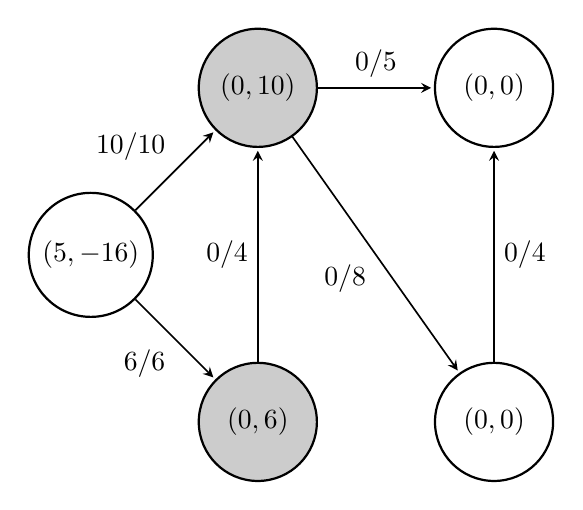
\begin{tikzpicture}[
            > = stealth, % arrow head style
            shorten > = 1pt, % don't touch arrow head to node set to +pt
            auto,
            node distance = 3cm, % distance between nodes
            semithick % line style
        ]

        \tikzstyle{every state}=[
            draw = black,
            thick,
            fill = white,
            minimum size = 15mm
        ]

        \node[state] (s) {$(5,-16)$};
        \node[state] (v1) [above right of=s, fill=gray!40] {$(0,10)$};
        \node[state] (v2) [below right of=s, fill=gray!40] {$(0,6)$};
        \node[state] (v3) [right of=v2] {$(0,0)$};
        \node[state] (t) [right of=v1] {$(0,0)$};

        \path[->] (s) edge node {$10/10$} (v1);
        \path[->] (s) edge node[below left] {$6/6$} (v2);
        \path[->] (v2) edge node[left] {$0/4$} (v1);
        \path[->] (v1) edge node[below left] {$0/8$} (v3);
        \path[->] (v1) edge node {$0/5$} (t);
        \path[->] (v3) edge node[right] {$0/4$} (t);

    \end{tikzpicture}

\end{document}
